\section{Apéndice: Análisis de Trazabilidad}

En esta sección realizamos un análisis de la trazabilidad de nuestro Trabajo
Práctico, siguiendo los lineamientos transmitidos por los docentes de la
materia.

Se presentan los mismos en un formato de tabla, para una mayor comodidad.

Para cada modelo, se buscó una forma de que sea fácil referenciar las partes
que consideramos atómicas, o importantes de mostrar (por ejemplo un objetivo
dentro de un Diagrama de Objetivos, o un Caso de Uso dentro del Modelo de
Casos de Uso, o incluso un paso dentro del mismo). Intentamos que las
referencias dentro de la tabla sean lo más intuitivas posibles, para evitar en
la medida de lo posible que necesiten de una explicación adicional.

Aunque no son un modelo, incluímos también una columna con los escenarios.
Esta columna no contiene <<todos>> los detalles, sino aquellos aspectos
representados en el texto que consideramos importantes mostrar.

También vale la pena hacer una mención especial sobre el significado de los
números en la columna de Actividad, que no es tan exacta como en el resto de
las columnas. En muchos casos, estamos representando actividades que están
relacionados, se desprenden, u ocasionan de algún modo, que se cumpla cierto
objetivo, o cierto fenómeno, y no necesariamente que haya una correspondencia
bidireccional entre la acción expresada en la fila y la actividad.

Tomamos distintos criterios para la granularidad de las acciones
representadas, la cual no es arbitraria, sino que responde a la propia
realización y documentación de la trazabilidad, actividad que nos obligó a
tener en mente en todo momento <<qué es lo que queríamos mostrar>> con el
nivel de granularidad elegido. Esta actividad de catalogar, enumerar y
documentar también nos permitió detectar inconsistencias o incoherencias entre
los distintos diagramas, particularmente entre el primer y el segundo
Trabajo Práctico.

El caso de uso 1.3 se debe interpretar como caso de uso 1, paso 3.
El diagrama conceptual no se traza por acciones puntuales, sino que abarca
conceptos transversales. Por eso no se lo incluye en este documento.
El modelo de contexto no permite agrupar eventos, por lo que no tiene
trazabilidad con eventos de más alto nivel como \texttt{Registro del cliente},
que sí están representados en los modelos de objetivos y de casos de uso.

A continuación se exponen los resultados del análisis descripto.

\begin{figure}[H]
	\begin{center}
	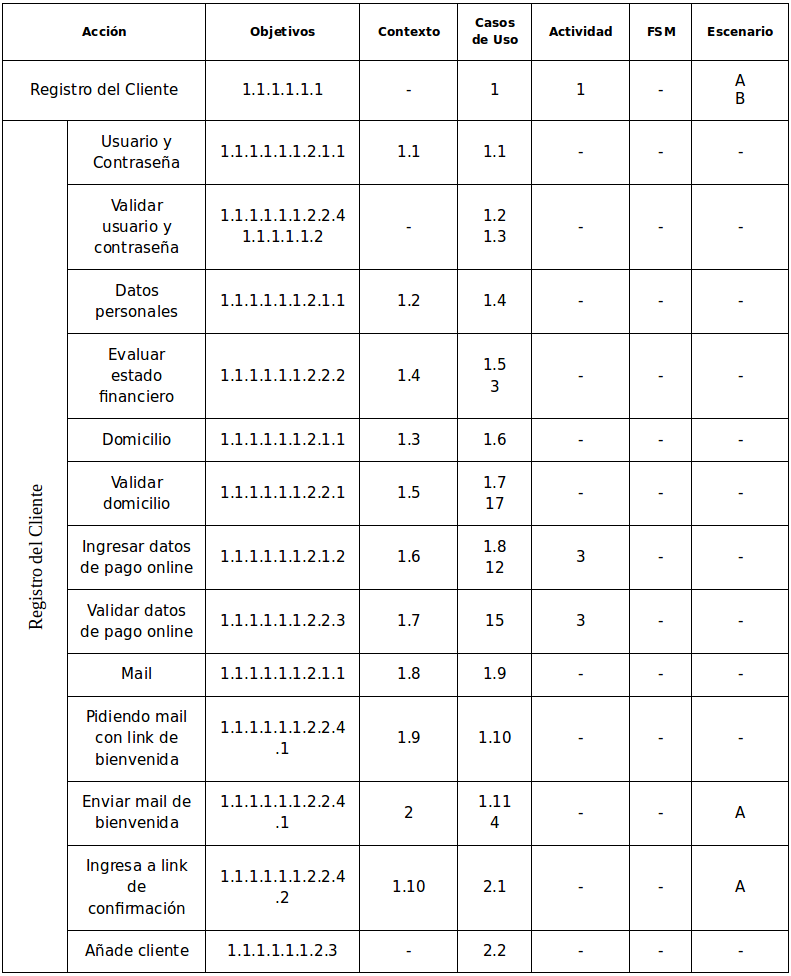
\includegraphics[width=\textwidth]{imagenes/trazabilidad-registro-cliente.png}
	\end{center}
	\label{trazabilidad-registro-cliente}
\end{figure}

\begin{figure}[H]
	\begin{center}
	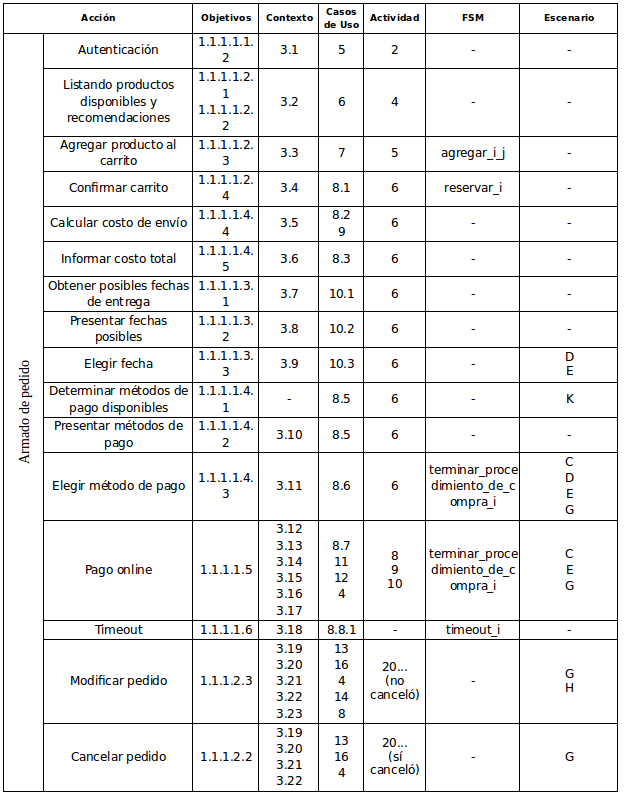
\includegraphics[width=\textwidth]{imagenes/trazabilidad-armado-pedido.png}
	\end{center}
	\label{trazabilidad-armado-pedido}
\end{figure}

\begin{figure}[H]
	\begin{center}
	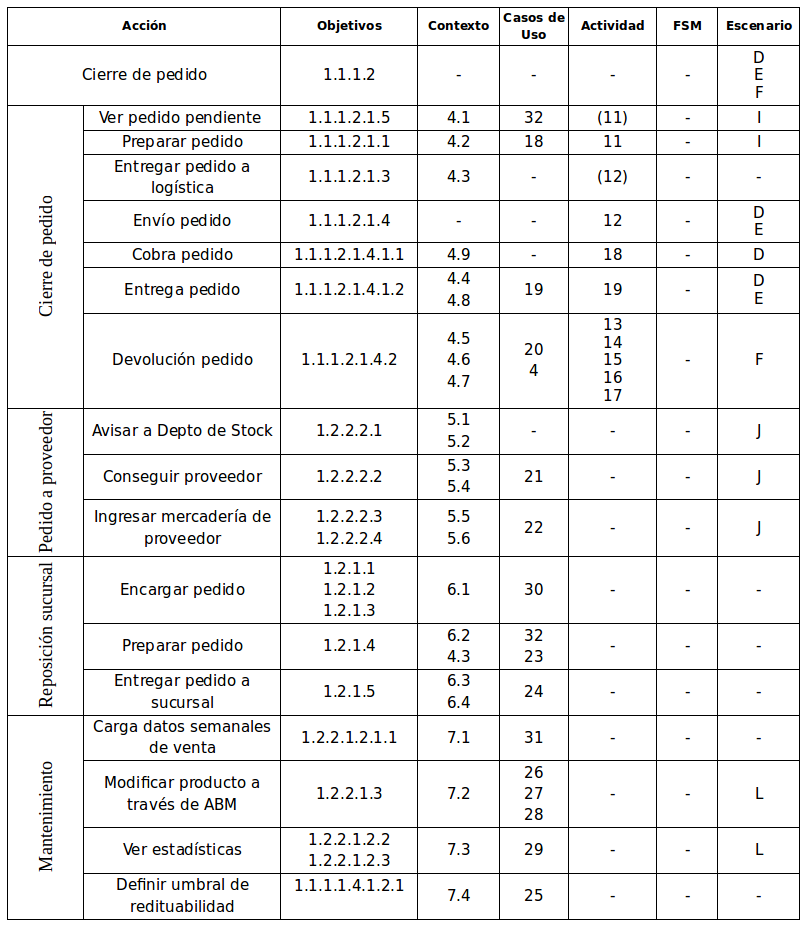
\includegraphics[width=\textwidth]{imagenes/trazabilidad-otros.png}
	\end{center}
	\label{trazabilidad-otros}
\end{figure}
